\documentclass{article}
\usepackage{geometry}
\usepackage{graphicx}
\usepackage{url}
\usepackage{hyperref}
\usepackage[spanish]{babel}
\usepackage{parskip}
\usepackage{amssymb}
\usepackage{float}

\title{High Level Computer Vision}

\author{
  \begin{minipage}[t]{0.4\linewidth}
    \centering
    Quistian Navarro, Juan Luis\\
    A341807@alumnos.uaslp.mx 
  \end{minipage}
}
\date{\today}
\begin{document}

\maketitle

\begin{minipage}{\textwidth}
  \centering
  \textit{Ing. Sistemas Inteligentes, Gen. 2021} \\
  \textit{Visión Computacional}
\end{minipage}

\small
\section*{Introducción}
En los últimos años, la visión por computadora ha experimentado un notable avance, lo que ha permitido el desarrollo de aplicaciones en campos como la robótica, los videojuegos, la seguridad, entre otros. Estos progresos han sido posibles gracias a la combinación de técnicas clásicas y modernas que van desde la detección de bordes hasta el uso de redes neuronales profundas. Este trabajo busca explorar y analizar diferentes enfoques de detección de objetos, haciendo énfasis en técnicas como la detección de bordes Canny, el algoritmo ORB (Oriented FAST and Rotated BRIEF) y los clasificadores Haar Cascade. Estas técnicas se han utilizado en una variedad de escenarios, como la detección de objetos en videojuegos y la identificación de patrones en imágenes y videos. En este documento, discutiremos las características y limitaciones de estos métodos, basándonos en su implementación práctica y resultados obtenidos.
\section{Videos}
\subsection*{Video 1: Canny Edge Detection y ORB Feature Matching - OpenCV Object Detection in Games}
\subsection*{Descripción del video y problema a resolver}
Este video muestra el intento del autor de implementar la detección de depósitos de piedra caliza en un videojuego usando dos técnicas clásicas de visión por computadora: la detección de bordes mediante el algoritmo de Canny y la coincidencia de características con ORB (Oriented FAST and Rotated BRIEF). El problema principal es que el autor busca identificar estos depósitos en diferentes condiciones de iluminación (ciclo día-noche), lo que hace que los métodos tradicionales de detección de bordes y características no funcionen de manera óptima.

\subsection*{Solución planteada}
El autor comienza implementando la detección de bordes de Canny para intentar identificar los contornos de los depósitos de piedra caliza. Sin embargo, al notar que esta técnica no ofrece buenos resultados debido a la variabilidad de las condiciones de luz, opta por usar ORB, un algoritmo más avanzado para la detección de características. ORB se selecciona debido a su eficiencia y porque es de código abierto, a diferencia de otros como SIFT y SURF.

\subsection*{Resolución del problema}
A lo largo del video, el autor ajusta varios parámetros en ambos métodos, como el tamaño del kernel en la erosión y dilatación de imágenes, y los umbrales de coincidencia de características en ORB. Sin embargo, aunque logra cierta mejora en la detección, el autor no alcanza una solución completamente efectiva. La técnica de detección de bordes sigue siendo limitada por la variabilidad en las condiciones del entorno, y la coincidencia de características con ORB tampoco es lo suficientemente robusta como para ofrecer resultados consistentes. Como posible solución, el autor sugiere que podría ser necesario recurrir a técnicas más avanzadas, como el aprendizaje automático.

\subsection*{Reflexión personal}
En mi opinión, este video muestra una interesante exploración de técnicas clásicas de visión por computadora aplicadas a un entorno complejo. Sin embargo, la limitación de estos métodos se hace evidente cuando se enfrentan a situaciones dinámicas como los cambios de iluminación. Aplaudo la creatividad del autor al probar diferentes enfoques y ajustar parámetros, aunque creo que, como él menciona, el aprendizaje automático sería un paso natural para resolver este tipo de problemas de manera más efectiva. Las redes neuronales convolucionales podrían ser una opción mucho más poderosa para lidiar con la variabilidad del entorno y proporcionar una detección más robusta.

\section*{Video 2: Entrenamiento de un Clasificador en Cascada - OpenCV Object Detection in Games}

\subsection*{Descripción del video y problema a resolver}
El segundo video trata sobre el entrenamiento de un clasificador en cascada para la detección de objetos en videojuegos. El autor busca demostrar cómo este método, aunque más sencillo que las redes neuronales profundas, puede ser efectivo para detectar objetos específicos, en este caso, depósitos de piedra caliza. El problema central que intenta resolver es la detección precisa de estos objetos en diversas condiciones del juego.

\subsection*{Solución planteada}
El autor comienza explicando el proceso de recopilación de imágenes positivas y negativas, esenciales para entrenar el clasificador en cascada. Usa capturas de pantalla del juego para obtener ejemplos de los objetos que desea detectar (positivos) y de objetos no deseados (negativos). Luego, utiliza una herramienta de anotación de OpenCV para crear archivos que describen las características de las imágenes positivas. Tras completar esta etapa, procede a entrenar el clasificador ajustando parámetros como el tamaño mínimo de las imágenes y el número de etapas de entrenamiento.

\subsection*{Resolución del problema}
El clasificador en cascada se entrena utilizando las imágenes anotadas, y tras varios intentos, el autor consigue que el modelo sea capaz de detectar los depósitos de piedra caliza de manera bastante precisa. A pesar de algunos falsos positivos y la necesidad de ajustar parámetros como el número de etapas, el modelo final parece funcionar de manera adecuada. El autor sugiere continuar experimentando con diferentes configuraciones para mejorar la precisión y evitar el sobreajuste, que es un problema común cuando se entrena con pocas imágenes o con un conjunto de datos desequilibrado.

\subsection*{Reflexión personal}
El video ofrece una explicación clara y accesible sobre cómo entrenar un clasificador en cascada, lo que resulta útil para quienes buscan una solución de detección de objetos sin recurrir a redes neuronales profundas. Aunque esta técnica tiene sus limitaciones en cuanto a la generalización y es susceptible a errores como falsos positivos, es una alternativa viable para problemas específicos de detección en tiempo real. En mi opinión, el uso de clasificadores en cascada es una buena opción cuando se cuenta con recursos computacionales limitados, pero a largo plazo, podría ser más eficiente utilizar redes neuronales más modernas, ya que permiten una mayor flexibilidad y precisión en la detección de objetos.

\section{Investigación}
\subsection*{Reconocimiento de objetos}
Es una técnica de visión artificial para identificar objetos en imágenes o en videos.
El reconocimiento de objetos constituye una salida clave de los algoritmos de deep learning y machine learning. Cuando las personas miramos una fotografía o vemos un video, detectamos con rapidez personas, objetos, lugares, y detalles visuales. El objetivo es enseñar a un ordenador a hacer lo que para nosotros resulta natural: adquirir cierto nivel de comprensión del contenido de una imagen \cite{mathworks_object_recognition}.

\begin{figure}[!ht]
  \centering
  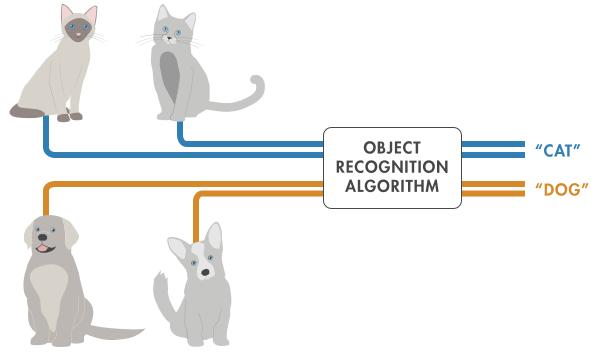
\includegraphics[width=0.65\linewidth]{images/ro.jpg}
  \caption{Utilización del reconocimiento de objetos para identificar distintas categorías de objetos.}
\end{figure}

\subsection*{Detector de bordes Canny}

En 1986, Canny propuso un método para la detección de bordes, el cual se basaba en tres criterios.

Uno de los métodos relacionados con la detección es el uso de la primera derivada, la que es usada por que toma el valor de cero en todas las regiones donde no varía la intensidad y tiene un valor constante en toda la transición de intensidad. Por tanto un cambio de intensidad se manifiesta como un cambio brusco en la primera derivada, característica que es usada para detectar un borde, y en la que se basa el algoritmo de Canny \cite{valdes_deteccion_bordes_canny}.

El algoritmo de Canny consiste en tres grandes pasos:

\begin{enumerate}
  \item Obtención del gradiente en este paso se calcula la magnitud y orientación del vector gradiente en cada pixel.
  \item Supresión no máxima, en este paso se logra el adelgazamiento del ancho de los bordes, obtenidos con el gradiente, hasta lograr bordes de un pixel ancho.
  \item Histéresis de umbral, en este paso se aplica una función de histéresis basada en dos umbrales; con este proceso se pretende reducir la posibilidad de aparición de contornos falsos.
\end{enumerate}

\begin{figure}[!ht]
  \centering
  \includegraphics[width=0.45\linewidth]{images/canny_conv.png}
  \caption{Mascaras de convolución para el filtro gaussiano}
\end{figure}

\begin{figure}[!ht]
  \centering
  \includegraphics[width=0.45\linewidth]{images/canny_intenisidad.png}
  \caption{Intensidad (maximización y minimización)}
\end{figure}

Resultados obtenidos de literatura, en donde aplican estos pasos para obtener los bordes canny:
\begin{figure}[!ht]
  \centering
  \includegraphics[width=0.45\linewidth]{images/canny_examples.png}
  \caption{Resultados de aplicar el detector de bordes de Canny: (a) imagen original; (b)
    orientación; (c) supresión no máxima; (d) histéresis de umbral.}
\end{figure}

\subsection*{Algoritmo de ORB}
Oriented Fast and Rotative Brief. Es un algoritmo desarrollado por OpenCV Labs, básicamente detecta puntos de puntos claves FAST (Features From Accelerated Segment Test) y construye el descriptor BRIEF (Binary Robust Independent Elementary Feature).
FAST es un método de detección de esquinas, que permite extraer puntos de características, que luego se utilizan para rastrear y mapear objetos, para cada pixel compara de manera rápida el brillo de ese pixel frente a 16 pixeles, los cuales forman un circulo alrededor del pixel p. Los pixeles en el circulo se clasifican en tres clases (más claras, más oscuras o similares) en caso de haber más de 8 pixeles más oscuros que p se selecciona como punto clave.

Los puntos claves o puntos de interés de una imagen son los puntos más relevantes de la misma, que a pesar de realizar alguna transformación no van a
cambiar.
Una limitación de FAST es que no tiene un componente de orientación o característica multiescala. Así es que ORB usa la pirámide de imágenes multiescala,
que es prácticamente la misma imagen en diferentes tamaños. Luego de detectar
los puntos claves, ORB asigna una orientación a cada punto clave, según cómo
cambien los niveles de intensidad alrededor del punto clave. BRIEF se construye
seleccionando todos los puntos claves encontrados de la imagen por el algoritmo
rápido FAST y los convierte en un vector de característica binario, definiendo
de esta manera un objeto \cite{core_detection_biomedical}.

\begin{figure}[!ht]
  \centering
  \includegraphics[width=0.35\linewidth]{images/ORB.png}
  \caption{Diagrama de flujo del algoritmo ORB}
\end{figure}

\subsection*{Clasificador Haar Cascade}
El clasificador Haar Cascade opera en una serie de etapas o cascadas. En cada etapa, se utilizan características simples que buscan distinguir entre el objeto objetivo y el fondo. Inicialmente, se aplican clasificadores más simples, y si la imagen pasa por todas las etapas, se considera que el objeto ha sido detectado. Esto reduce significativamente el tiempo de procesamiento, ya que las imágenes que no contienen el objeto son descartadas en las primeras etapas.

Para entrenar un clasificador Haar, se necesita un conjunto de imágenes positivas, que contienen el objeto que se desea detectar, y un conjunto de imágenes negativas, que no lo contienen. El proceso de entrenamiento ajusta los umbrales y parámetros del clasificador para que sea capaz de distinguir entre los objetos de interés y el fondo con alta precisión.

Aunque el clasificador Haar Cascade ha sido utilizado con éxito en la detección de rostros y otros objetos, presenta ciertas limitaciones, como la sensibilidad a la variación en las condiciones de iluminación y la necesidad de un número considerable de imágenes para el entrenamiento. A pesar de estas limitaciones, sigue siendo una herramienta valiosa en la visión por computadora debido a su simplicidad y velocidad de procesamiento en tiempo real \cite{omesva_deteccion_rostros_haar}.

\begin{figure}[!ht]
  \centering
  \includegraphics[width=0.45\linewidth]{images/Haar-cascade.png}
  \caption{Proceso para crear un clasificador de rostros empleando Haar-Cascade}
\end{figure}

\section*{Conclusión}
La visión por computadora ofrece diversas técnicas para la detección de objetos, como el detector de bordes de Canny, ORB y los clasificadores Haar Cascade. Aunque estos métodos presentan limitaciones frente a variaciones en el entorno, siguen siendo útiles en aplicaciones de bajo costo computacional. A futuro, el uso de redes neuronales profundas mejorará significativamente la precisión y flexibilidad en la detección de objetos, complementando o reemplazando a los métodos tradicionales.

\bibliographystyle{plain}
\bibliography{ref}
\end{document}
